\documentclass[12pt]{article}

\usepackage[hidelinks]{hyperref}
\usepackage{graphicx}
\usepackage{color}
\usepackage{xcolor}
\usepackage{listings}
\usepackage{courier}

% syntax highlighting from: http://www.kv0.org/blog/2010/12/15/vernunftiges-syntax-highlighting-in-latex/
\lstset{
	basicstyle=\footnotesize\ttfamily, % Standardschrift
	numbers=left, % Ort der Zeilennummern
	numberstyle=\tiny, % Stil der Zeilennummern
	%stepnumber=2, % Abstand zwischen den Zeilennummern
	numbersep=5pt, % Abstand der Nummern zum Text
	tabsize=2, % Groesse von Tabs
	extendedchars=true, %
	breaklines=true, % Zeilen werden Umgebrochen
	keywordstyle=\color{orange}\bfseries,
	frame=b,
	% keywordstyle=[1]\textbf, % Stil der Keywords
	% keywordstyle=[2]\textbf, %
	% keywordstyle=[3]\textbf, %
	% keywordstyle=[4]\textbf, \sqrt{\sqrt{}} %
	stringstyle=\color{white}\ttfamily, % Farbe der String
	showspaces=false, % Leerzeichen anzeigen ?
	showtabs=false, % Tabs anzeigen ?
	xleftmargin=17pt,
	framexleftmargin=17pt,
	framexrightmargin=5pt,
	framexbottommargin=4pt,
	commentstyle=\color{green},
	% backgroundcolor=\color{gray},
	showstringspaces=false, % Leerzeichen in Strings anzeigen ?
	morekeywords={__global__} % CUDA specific keywords
}
\lstloadlanguages{% Check Dokumentation for further languages ...
%[Visual]Basic
%Pascal
C,
C++,
%XML
%HTML
Java
}
%\DeclareCaptionFont{blue}{\color{blue}}
 
%\captionsetup[lstlisting]{singlelinecheck=false, labelfont={blue}, textfont={blue}}
\usepackage{caption}
\DeclareCaptionFont{white}{\color{white}}
\DeclareCaptionFormat{listing}{\colorbox{gray}{\parbox{\textwidth}{\hspace{15pt}#1#2#3}}}
\captionsetup[lstlisting]{format=listing,labelfont=white,textfont=white, singlelinecheck=false, margin=0pt, font={bf,footnotesize}}

\title{Project Report - First assignment - GAME ENGINES}
\author{Andrea Distler}
\date{28 November, 2012}

\begin{document}
\maketitle
\newpage

\tableofcontents
\newpage

%------------------------------------------
\section{Introduction}
This is the project report for the first assignment of the Game Engines course.

A short description of the source code and the used libraries can be found in section \ref{section:files}. The files are available on GitHub. The libraries are also made available on GitHub for easier installation.

Section \ref{section:outcome} describes the outcome of the project. 

Section\ref{section:overview} gives an overview of the used mechanics and points out the key features of the project. 

Section \ref{section:classes} gives a detailed description of the important classes and their relations to each other. It also points out challenging parts of the code.

I have invested an unnecessarily big amount of time into this small assignment, and I want to elaborate on my workflow in section \ref{section:workflow}.

%------------------------------------------
\section{The Files}
\label{section:files}
All files can be found on GitHub. \newline 
\url{https://github.com/JungleJinn/GE---SimplePlatformerEngine}.

\subsection{Used Libraries}

The project was written in C++, using additional libraries:

\begin{itemize}
\item{
	Included in the repository
	\begin{itemize}
		\item{SDL image}
	\end{itemize}
}

\item{
	External
	\begin{itemize}
		\item{openGL. Installed manually. Files in zip}
		\item{glm. Installed manually. Files in zip}
		\item{SDL 1.2.15. \url{http://www.libsdl.org/download-1.2.php} Used environment variable named SDK\_SDL}
	\end{itemize}
}
\end{itemize}

%------------------------------------------
\section{Outcome}
\label{section:outcome}

The project's result is a little game in which the player can control a bomb. The player cannot directly control the bomb's position. However, it is possible to change the bomb's mass and therefore indirectly possible to steer the bomb. The goal of the game is to survive as long as possible, which is made hard by other bombs which present themselves as obstacles. Depending on the player's mass, the enemy bomb will affect the player's further movement. If the player moves backwards, the game is over. For a screenshot of the game see figure \ref{figure:outcome}.

There is a short explanation of the controls and rules of the game in the beginning. Once a player loses, there is also a gameover screen, telling the player that the game is now over.

The assignment was to create a simple physics engine which can be used for a platformer. The game features:

\begin{itemize}
	\item{2D physics}
	\item{openGL rendering}
	\item{an intro screen and an outro screen}
	\item{a dragon with a hat}
	\item{sprites and texture atlases}
	\item{collision detection and response}
	\item{bounciness}
	\item{very intuitive controls}
\end{itemize}

\begin{figure}[H]
	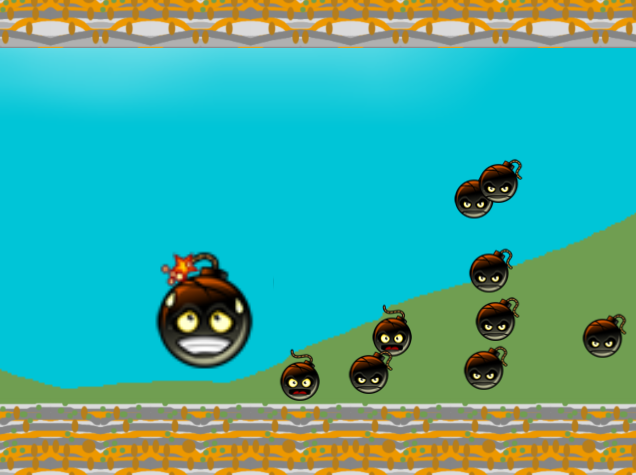
\includegraphics[width=\textwidth]{outcome.png}
	\caption{A screenshot of the game.}
	\label{figure:outcome}
\end{figure}

% -----------------------------------------
\section{Overview}
\label{section:overview}

This section gives an overview over used mechanics.

\subsection{Game Loop}

\begin{lstlisting}[caption=The game loop, language=C++]
lastUpdateTime = clock();
Init();

quit = false;
while (!quit)
{
	Play();
}
\end{lstlisting}

First the game is being set up, then the game loop starts. The game loop is quite basic. While the game has not been quit, it is playing.\newline

\subsection{Messaging}

The Input is realized by using SDL events. The first thing done in the Play method is to fetch all pending input events. These events are then sorted by what is important, what is to be used in the game, and what not. Then the newly written message system starts to create and forward messages.

\begin{lstlisting}[caption=Messaging, language=C++]
SDL_Event sdlEvent = SDL_Event();
while (SDL_PollEvent(&sdlEvent))
{
	// user closes window
	if (sdlEvent.type == SDL_QUIT)
	{
		quit = true;
		break;
	}
	else if (sdlEvent.type == SDL_KEYDOWN)
	{
		messenger->SendMessage(InputMessage(InputMessage::KEY_DOWN, sdlEvent.key.keysym.sym));
	}
	else if (sdlEvent.type == SDL_KEYUP)
	{
		messenger->SendMessage(InputMessage(InputMessage::KEY_UP, sdlEvent.key.keysym.sym));
	}
}
\end{lstlisting}

The messenger can send messages of different types to receivers of type IMessageReceiver. All objects of this type automatically register and unregister at the messenger at creation and deletion. The receivers decide which kinds of messages they want to process, but each receiver gets all sent messages.

\subsection{Physics}

The physics are calculated in two dimensions. The physics system is responsible for movement and for collisions as well as for collision response. Bodies are implemented as simple rigid bodies. Forces can be applied. There are two basic collision shapes: Circles and Rectangles. The collision detection happens in two states, first the broad phase, which only checks the radius of the objects, and the narrow phase, in which the collision normal is calculated. The normal is then used to determine the resulting forces acting on both colliders. Bodies have a coefficient of restitution which adds to the collision response. The combination method is to use the average coefficient of restitution of both bodies.

For integrating forces, the integration method receives a value named deltaTime. The delta time is calculated like in the following listing:

\begin{lstlisting}[caption=deltaTime, language=C++]
int now = clock();
deltaTime = (float)((now - lastUpdateTime) / CLOCKS_PER_SEC) / timeScale;
lastUpdateTime = now;
\end{lstlisting}

The whole game execution can be slowed or fastened by setting different timeScale values. At a value of 1.0 it is executed in real-time, and other values stretch or squish the perceived time.

\subsection{Sprites}

Sprites are used for the player and for the enemy bombs. They are stored in a spritesheet and their texture coordinates are adapted to fit certain sprite frames.

\subsection{Camera}

The camera is moving with the player all the time. A problem encountered with a potentially endless level was whether the floor and ceiling should always be recreated. The player can move as far as he wants to, therefore an inifinite amount of rectangular walls would be needed. The solution which avoids creating endless amounts of floor tiles was to always move the floor and ceiling with the player (not unlike the camera). The texture coordinates change to create the visual feedback of the player's velocity. The illusion that the player moves in relation to the floor is created, whereas the player and the floor have a relative velocity of zero. The background also follows the player.

\subsection{Dragon}

In the first phase of the game the player can choose the launch angle by rotating a dragon's head.

%-----------------------------------------
\section{Important Classes}
\label{section:classes}

In figure \ref{figure:classes} a selection of classes is depicted.

\paragraph{Game.}
The game class manages the game states and 

\begin{figure}[H]
	\centering
	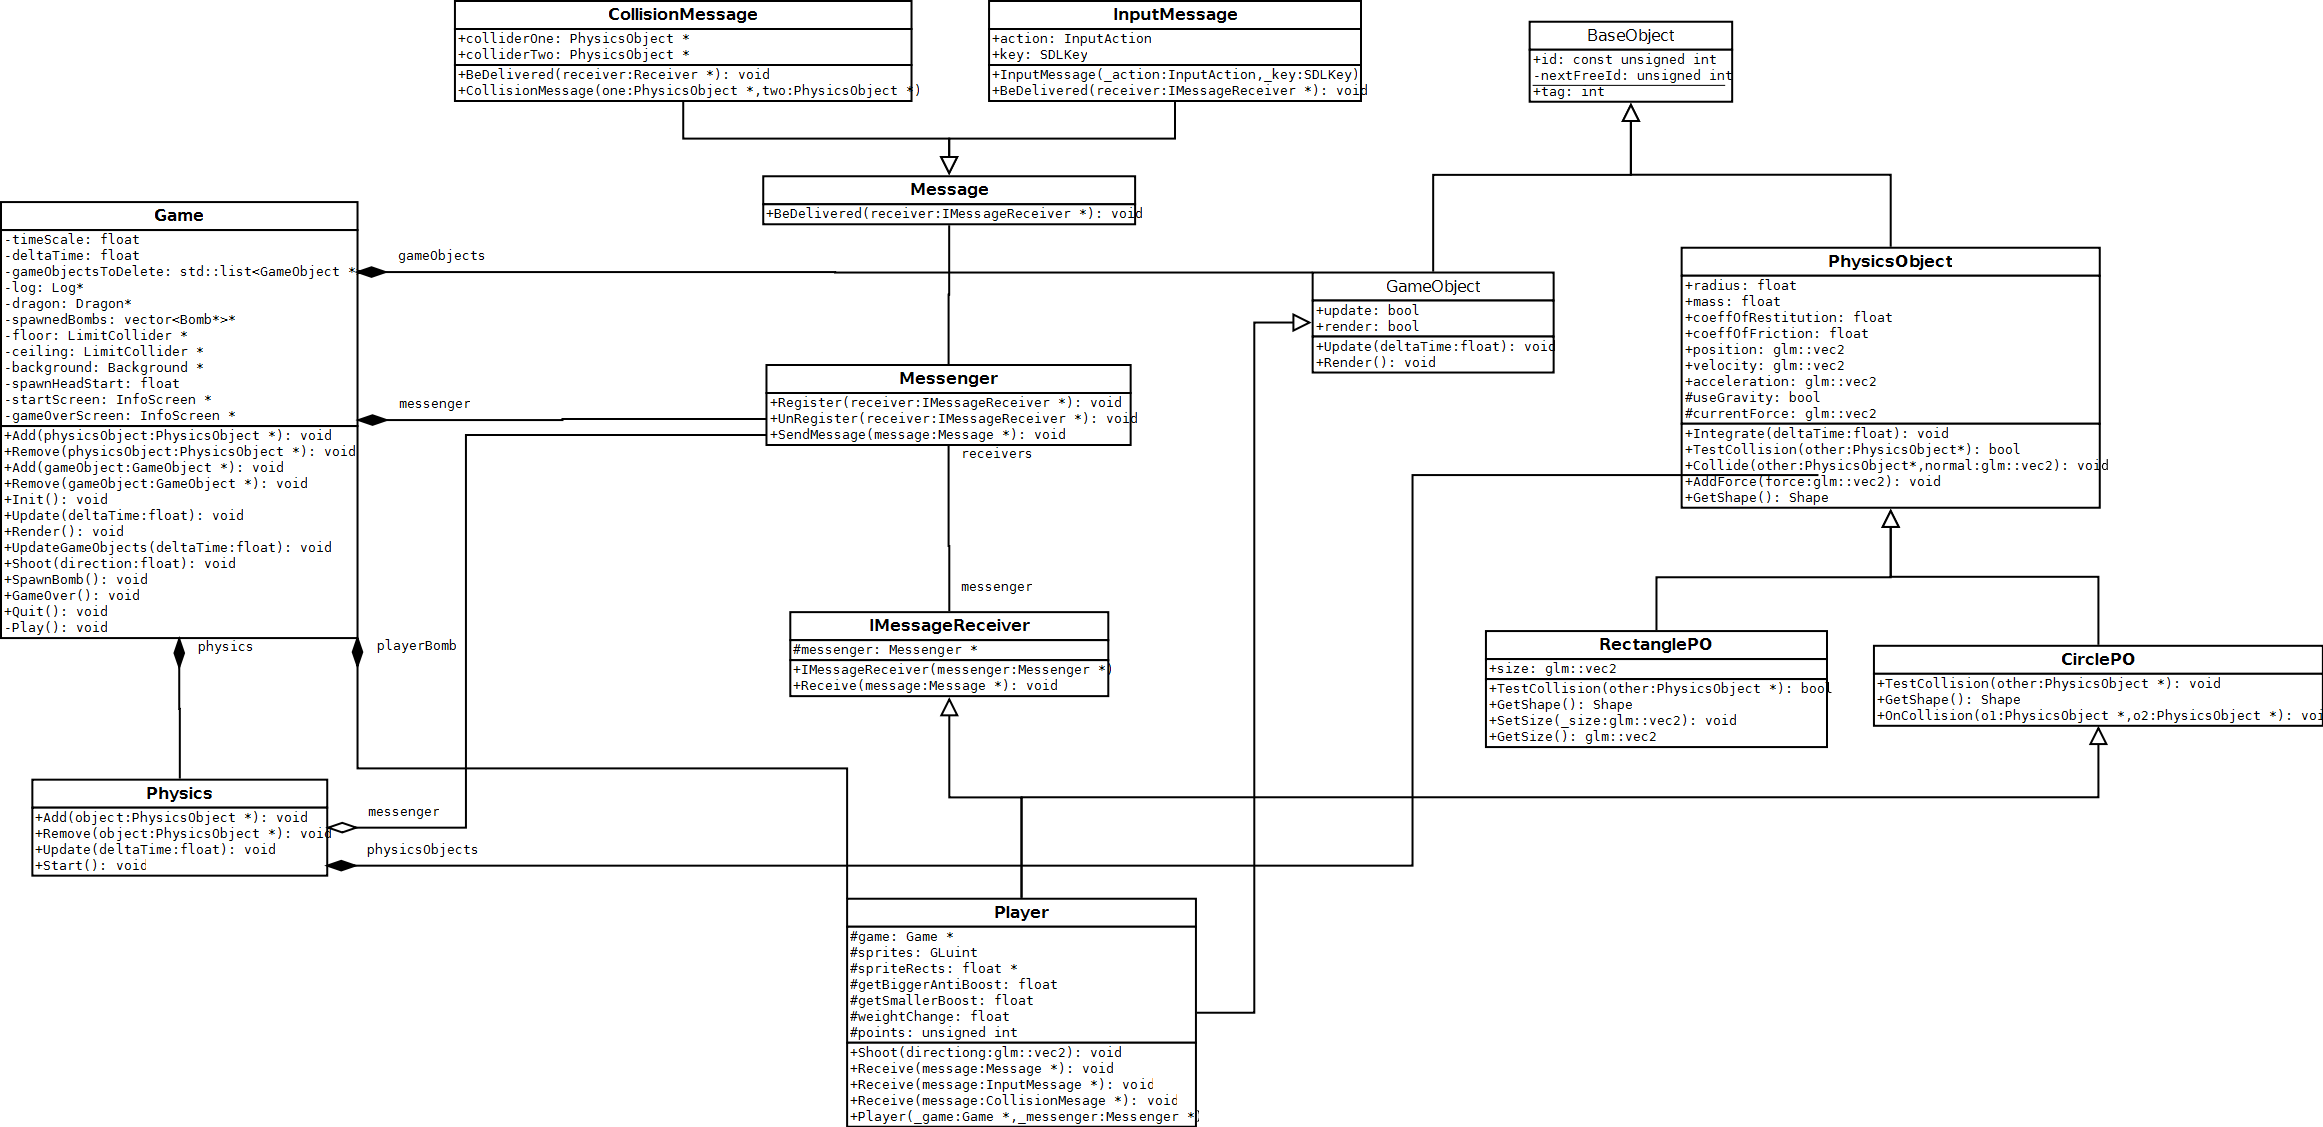
\includegraphics[totalheight=0.5\textheight, angle=90]{classes.png}
	\caption{A sketch of the most important classes.}
	\label{figure:classes}
\end{figure}

%-----------------------------------------
\section{Workflow}
\label{section:workflow}

\newpage
\lstlistoflistings
\listoffigures

\end{document}